% Two-stage architecture figure for the symposium poster, drawn in TikZ.
%
% Build (from this directory):
%   ./build_architecture.sh
%
% Everything graph-shaped in this figure is ONE graph: a real 30-voxel ball of
% one Duke case's centerline network, extracted once by
% analysis/poster_architecture_data.py into architecture_data/graph.tex and
% redrawn from the same stored coordinates at every stage. A reader can follow
% the same branch from the MRI, through per-frame message passing, to the
% forecast target and on into the pCR head. Nothing here is a generic blob
% standing in for "a graph".
%
% The MRI panels are real DCE-MRI frames from the public MAMA-MIA Duke cohort --
% not UChicago, whose slices must not be printed on a public poster.
%
% The forecast panel shades nodes by the *measured* enhancement at the target
% frame. No forecaster is run to make this figure, so it shows the target field
% the decoder is trained on rather than a prediction it did not produce.

\documentclass[tikz,border=3pt]{standalone}

\usepackage{fontspec}
\usepackage{pgfplots}
\pgfplotsset{compat=1.14}
\usetikzlibrary{arrows.meta, backgrounds, calc, fit, positioning, shapes.geometric}

% Poster palette. Maroon/light maroon come from beamercolorthemeuchicago.sty;
% node blue and edge orange match the pipeline figure so a graph node is the
% same colour everywhere on the poster.
\definecolor{maroon}{RGB}{128, 0, 0}
\definecolor{darkmaroon}{RGB}{91, 0, 0}
\definecolor{lightmaroon}{RGB}{250, 236, 236}
\definecolor{nodeblue}{RGB}{63, 167, 255}
\definecolor{edgeorange}{RGB}{230, 126, 34}
\definecolor{ink}{RGB}{40, 40, 40}
\definecolor{slate}{RGB}{107, 114, 128}
\definecolor{panel}{RGB}{244, 244, 246}

% Generated by analysis/poster_architecture_data.py -- do not edit.
% One real vessel subgraph, shared by every panel of the architecture figure.

\def\voxelnodes{0.0000/0.3862, 0.0892/0.3895, 0.1960/0.3208, 0.1489/0.3453, 0.2557/0.2766, 0.3450/0.2799, 0.6527/0.0933, 0.6056/0.1178, 0.8065/0.0000, 0.7594/0.0245, 0.7124/0.0491, 0.5283/0.2341, 0.4813/0.2587, 0.4342/0.2832, 0.5880/0.1899, 0.2031/0.4928, 0.2628/0.4486, 0.4637/0.3308, 0.3696/0.3799, 0.3225/0.4044, 0.4806/0.3979, 0.4336/0.4225, 0.5572/0.4209, 0.6465/0.4242, 0.7231/0.4472, 0.7997/0.4702, 0.8637/0.5128, 0.9403/0.5358, 1.0000/0.4916, 0.9572/0.6030}
\def\voxelheatA{21, 21, 21, 21, 21, 21, 21, 21, 21, 21, 21, 21, 21, 21, 21, 21, 21, 21, 21, 21, 21, 21, 21, 21, 21, 21, 21, 21, 21, 21}
\def\voxelheatB{35, 44, 70, 53, 51, 70, 85, 74, 47, 43, 68, 77, 52, 52, 65, 84, 88, 66, 49, 97, 18, 27, 87, 28, 75, 28, 35, 48, 17, 77}
\def\voxelheatC{61, 67, 100, 96, 27, 63, 48, 62, 53, 56, 49, 52, 72, 72, 44, 56, 54, 72, 61, 93, 27, 66, 47, 56, 56, 29, 34, 68, 21, 32}
\def\voxelheatD{10, 24, 44, 36, 28, 54, 26, 14, 19, 37, 28, 49, 59, 25, 46, 17, 0, 29, 37, 30, 36, 36, 30, 12, 30, 2, 41, 37, 20, 26}
\def\voxelheatE{63, 45, 69, 85, 54, 83, 35, 48, 29, 33, 40, 83, 64, 33, 66, 51, 82, 66, 38, 58, 81, 74, 88, 60, 61, 26, 45, 37, 30, 56}
\def\voxelheat{63, 45, 69, 85, 54, 83, 35, 48, 29, 33, 40, 83, 64, 33, 66, 51, 82, 66, 38, 58, 81, 74, 88, 60, 61, 26, 45, 37, 30, 56}
\def\voxeledges{0/1, 3/1, 3/2, 4/5, 4/2, 6/10, 7/6, 9/10, 9/8, 12/17, 12/11, 12/13, 13/5, 14/7, 14/11, 16/15, 17/13, 18/21, 18/19, 19/16, 20/17, 20/22, 21/17, 21/20, 23/22, 23/24, 24/25, 26/25, 27/29, 27/26, 28/27}
\def\junctionnodes{0.0000/0.3862, 0.8065/0.0000, 0.4813/0.2587, 0.4342/0.2832, 0.2031/0.4928, 0.4637/0.3308, 0.4806/0.3979, 0.4336/0.4225, 0.9403/0.5358, 1.0000/0.4916, 0.9572/0.6030}
\def\junctionedges{7/4, 7/5, 7/6, 0/3, 2/5, 2/1, 2/3, 6/5, 6/8, 9/8, 8/10, 5/3}
\def\segmentnodes{0.3225/0.4044, 0.4637/0.3308, 0.4806/0.3979, 0.1960/0.3208, 0.4637/0.3308, 0.6527/0.0933, 0.4342/0.2832, 0.4637/0.3308, 0.7231/0.4472, 0.9403/0.5358, 0.9572/0.6030, 0.4342/0.2832}
\def\segmentedges{0/1, 0/2, 1/2, 1/4, 1/7, 1/11, 2/7, 2/8, 3/6, 3/11, 4/5, 4/6, 4/7, 4/11, 5/6, 6/11, 7/8, 7/11, 8/9, 8/10, 9/10}
\def\segmentpathA{(0.4336,0.4225) (0.3696,0.3799) (0.3225,0.4044) (0.2628,0.4486) (0.2031,0.4928)}
\def\segmentpathB{(0.4336,0.4225) (0.4637,0.3308)}
\def\segmentpathC{(0.4336,0.4225) (0.4806,0.3979)}
\def\segmentpathD{(0.0000,0.3862) (0.0892,0.3895) (0.1489,0.3453) (0.1960,0.3208) (0.2557,0.2766) (0.3450,0.2799) (0.4342,0.2832)}
\def\segmentpathE{(0.4813,0.2587) (0.4637,0.3308)}
\def\segmentpathF{(0.4813,0.2587) (0.5283,0.2341) (0.5880,0.1899) (0.6056,0.1178) (0.6527,0.0933) (0.7124,0.0491) (0.7594,0.0245) (0.8065,0.0000)}
\def\segmentpathG{(0.4813,0.2587) (0.4342,0.2832)}
\def\segmentpathH{(0.4806,0.3979) (0.4637,0.3308)}
\def\segmentpathI{(0.4806,0.3979) (0.5572,0.4209) (0.6465,0.4242) (0.7231,0.4472) (0.7997,0.4702) (0.8637,0.5128) (0.9403,0.5358)}
\def\segmentpathJ{(1.0000,0.4916) (0.9403,0.5358)}
\def\segmentpathK{(0.9403,0.5358) (0.9572,0.6030)}
\def\segmentpathL{(0.4637,0.3308) (0.4342,0.2832)}
\def\segmentcount{12}

% Generated by analysis/poster_architecture_data.py -- do not edit.
% Real baseline-referenced DCE enhancement at selected graph nodes.

\def\curveobsA{(0,0.0000) (1,0.6206) (2,1.0000)}
\def\curvefutA{(2,1.0000) (3,0.2914) (4,0.6115)}
\def\curveobsB{(0,0.0000) (1,0.4112) (2,0.9530)}
\def\curvefutB{(2,0.9530) (3,0.1973) (4,0.8103)}
\def\curveobsC{(0,0.0000) (1,0.9621) (2,0.9165)}
\def\curvefutC{(2,0.9165) (3,0.1168) (4,0.4689)}
\def\curveinputlen{3}
\def\curvetotallen{5}
\def\curvelastinput{2}
\def\framelist{00,01,02,03,04}


% ---------------------------------------------------------------------------
% The shared graph.
%
% \placegraph lays the stored unit coordinates into named TikZ coordinates under
% a prefix, so the same graph can appear many times in one picture without its
% node names colliding. The \...graph macros then stroke one prefix. Scale is
% the only thing that differs between appearances.
% ---------------------------------------------------------------------------
\newcommand{\placegraph}[2]{%
  \foreach \gx/\gy [count=\i from 0] in \voxelnodes {%
    \coordinate (#1-\i) at ({\gx*#2},{\gy*#2});%
  }%
}
\newcommand{\graphedges}[2]{%
  \foreach \a/\b in \voxeledges {\draw[#2] (#1-\a) -- (#1-\b);}%
}

% Full-size appearance: orange edges, blue nodes.
\newcommand{\bigraph}[2]{%
  \placegraph{#1}{#2}%
  \graphedges{#1}{edgeorange, line width=1.6pt}%
  \foreach \gx/\gy [count=\i from 0] in \voxelnodes {\fill[nodeblue] (#1-\i) circle (3.0pt);}%
}
% Small appearance, for the per-frame plates inside the encoder. Node shading
% is that frame's measured enhancement, on one scale shared by every frame, so
% the plates differ in exactly the way the real input does: same topology, same
% positions, different node values.
\newcommand{\minigraph}[3]{% prefix, scale, per-frame shading macro
  \placegraph{#1}{#2}%
  \graphedges{#1}{slate!40, line width=1.0pt}%
  \foreach \v [count=\i from 0] in #3 {\fill[maroon!\v!nodeblue] (#1-\i) circle (1.8pt);}%
}
% Forecast-target appearance: node shading is the measured enhancement field.
\newcommand{\heatgraph}[2]{%
  \placegraph{#1}{#2}%
  \graphedges{#1}{slate!45, line width=1.4pt}%
  \foreach \v [count=\i from 0] in \voxelheat {\fill[maroon!\v!nodeblue] (#1-\i) circle (3.0pt);}%
}

\tikzset{
  procbox/.style={
    draw=maroon, fill=white, line width=1.4pt, rounded corners=5pt,
    align=center, inner sep=7pt, text=ink, font=\sffamily\fontsize{16}{19}\selectfont,
  },
  darkbox/.style={
    draw=maroon, fill=maroon, line width=1.4pt, rounded corners=5pt,
    align=center, inner sep=7pt, text=white,
    font=\sffamily\bfseries\fontsize{16}{19}\selectfont,
  },
  plate/.style={draw=slate!35, fill=white, line width=0.9pt, rounded corners=3pt},
  panelbox/.style={draw=slate!40, fill=white, line width=1pt, rounded corners=5pt},
  encoderbox/.style={
    draw=maroon, fill=white, line width=1.6pt, rounded corners=8pt,
    dash pattern=on 10pt off 5pt,
  },
  flow/.style={-{Stealth[length=9pt, width=7pt]}, line width=1.8pt, draw=slate},
  transfer/.style={
    -{Stealth[length=10pt, width=8pt]}, line width=2.4pt, draw=maroon,
  },
  caption/.style={font=\sffamily\fontsize{14}{16}\selectfont, text=ink, align=center},
  note/.style={font=\sffamily\fontsize{12}{14}\selectfont, text=slate, align=center},
  stagetitle/.style={
    font=\sffamily\bfseries\fontsize{18}{21}\selectfont, text=maroon, align=left,
  },
}

\begin{document}
\begin{tikzpicture}[x=1cm, y=1cm]

% ===========================================================================
% STAGE 1 -- self-supervised forecasting on the unlabeled pool
% ===========================================================================
\begin{scope}[on background layer]
  \fill[lightmaroon, rounded corners=10pt] (-0.6, 5.75) rectangle (27.2, 14.6);
\end{scope}

\node[stagetitle, anchor=west] at (-0.2, 14.15)
  {1.\ \ PRETRAIN\ \textemdash\ 1{,}226 unlabeled exams, no pCR label used};

% --- The real DCE-MRI movie -------------------------------------------------
\foreach \f [count=\k from 0] in \framelist {%
  \node[inner sep=0pt] at ({0.9 + \k*1.66}, 12.5)
    {\includegraphics[width=1.55cm]{architecture_data/mri_frame_\f.png}};%
}
\node[caption, anchor=north] at (4.2, 11.55) {ultrafast DCE-MRI movie};
\node[note, anchor=north, text width=6.2cm] at (4.2, 11.05) {one frame per acquisition time};
\draw[flow] (8.6, 12.5) -- (9.2, 12.5);

% --- The centerline, on the image it came from ------------------------------
\node[inner sep=0pt] at (10.8, 12.5)
  {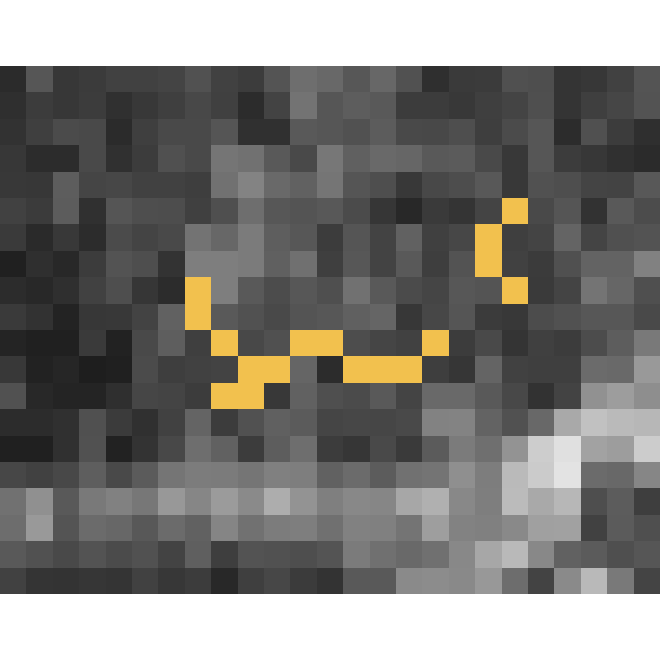
\includegraphics[width=2.7cm]{architecture_data/mri_centerline.png}};
\node[caption, anchor=north] at (10.8, 11.55) {vessel centerline};
\node[note, anchor=north, text width=3.4cm] at (10.8, 11.05) {nnU-Net, then tc4d};
\draw[flow] (12.45, 12.5) -- (13.05, 12.5);

% --- The graph: first appearance of the object the reader then follows ------
\begin{scope}[shift={(13.35, 11.75)}]
  \bigraph{gA}{2.9}
\end{scope}
\node[caption, anchor=north] at (14.8, 11.55) {vessel-network graph};
\node[note, anchor=north, text width=4.4cm] at (14.8, 11.05) {one node per centerline voxel};

% --- What every node carries ------------------------------------------------
\node[panelbox, minimum width=8.6cm, minimum height=3.2cm] at (22.6, 12.6) {};
\begin{scope}[shift={(19.4, 11.5)}]
  \begin{axis}[
      at={(0,0)}, anchor=south west, width=6.6cm, height=1.9cm,
      scale only axis, xmin=0, xmax=\curvetotallen-1, ymin=-0.35, ymax=1.15,
      axis line style={draw=slate}, tick style={draw=slate},
      xtick=\empty, ytick=\empty, axis y line=left, axis x line=bottom,
      clip=false,
    ]
    % Solid = the input horizon the encoder sees; dashed = what it must predict.
    \addplot[nodeblue, line width=1.7pt] coordinates {\curveobsA};
    \addplot[nodeblue, line width=1.7pt, densely dashed] coordinates {\curvefutA};
    \addplot[edgeorange, line width=1.7pt] coordinates {\curveobsB};
    \addplot[edgeorange, line width=1.7pt, densely dashed] coordinates {\curvefutB};
    \addplot[maroon, line width=1.7pt] coordinates {\curveobsC};
    \addplot[maroon, line width=1.7pt, densely dashed] coordinates {\curvefutC};
    \draw[slate, dotted, line width=1.3pt]
      (axis cs:\curvelastinput,-0.35) -- (axis cs:\curvelastinput,1.15);
  \end{axis}
\end{scope}
\node[caption, anchor=south] at (22.6, 14.3) {measured enhancement at three of its nodes};
\node[note, anchor=north] at (20.6, 11.4) {frames seen};
\node[note, anchor=north] at (25.0, 11.4) {frames forecast};

% The curves belong to the graph on the left, not to a separate object.
\draw[slate!60, line width=1.1pt, dashed] (16.4, 12.5) -- (18.2, 12.5);

% --- Into the encoder -------------------------------------------------------
\draw[flow] (14.8, 10.4) -- (14.8, 9.98);

% ===========================================================================
% The encoder: the only thing whose weights transfer
% ===========================================================================
\node[encoderbox, minimum width=19.2cm, minimum height=3.9cm] at (9.9, 8.0) {};
\node[darkbox, anchor=north west] at (0.45, 9.8) {shared graph encoder};
\node[note, anchor=north west, text width=4.3cm, align=left] at (0.5, 8.75)
  {inputs: node curves,\\ graph edges, elapsed times};

\node[caption, anchor=north] at (12.4, 9.85) {one GCN pass per frame, over the same graph};

% Unrolled, not a \foreach: pgffor expands its list items, and a shading macro
% expands to a comma-separated list, which would tear the outer list apart.
\newcommand{\gcnplate}[3]{% x centre, prefix, shading macro
  \node[plate, minimum width=2.7cm, minimum height=2.15cm] at (#1, 8.0) {};
  \begin{scope}[shift={(#1 - 1.1, 7.3)}]
    \minigraph{#2}{2.2}{#3}
  \end{scope}%
}
\gcnplate{6.0}{gcnA}{\voxelheatA}
\gcnplate{9.2}{gcnB}{\voxelheatB}
\gcnplate{13.8}{gcnC}{\voxelheatE}
\node[note] at (11.5, 8.0) {$\cdots$};
\node[note, anchor=north] at (6.0, 6.75) {frame 1};
\node[note, anchor=north] at (13.8, 6.75) {frame $T$};

\node[procbox, minimum width=2.5cm, minimum height=1.8cm] at (17.2, 8.0)
  {GRU\\ per node};
\draw[flow] (15.2, 8.0) -- (15.9, 8.0);
\node[note, anchor=north, text width=4.6cm] at (17.2, 6.75)
  {one hidden state per node};

% --- Decoder and the forecast target ----------------------------------------
\node[procbox, minimum width=3.1cm, minimum height=1.8cm] at (21.6, 8.0)
  {forecasting\\ decoder};
\draw[flow] (18.5, 8.0) -- (20.0, 8.0);
\draw[flow] (23.2, 8.0) -- (23.95, 8.0);

\begin{scope}[shift={(24.25, 7.3)}]
  \heatgraph{gB}{2.4}
\end{scope}
\node[caption, anchor=north, text width=5.6cm] at (25.45, 7.1)
  {enhancement at every node,\\ at times it was never shown};

% ===========================================================================
% Transfer
% ===========================================================================
\draw[transfer] (6.6, 6.0) -- (6.6, 4.85);
\node[stagetitle, anchor=west] at (6.95, 5.4) {transfer encoder weights};

% ===========================================================================
% STAGE 2 -- fine-tuning on the labeled cohort
% ===========================================================================
\begin{scope}[on background layer]
  \fill[panel, rounded corners=10pt] (-0.6, -1.15) rectangle (27.2, 4.6);
\end{scope}

\node[stagetitle, anchor=west] at (-0.2, 4.15)
  {2.\ \ FINE-TUNE\ \textemdash\ 179 labeled exams, patient-grouped folds};

\draw[transfer, dash pattern=on 8pt off 5pt] (6.6, 3.65) -- (6.6, 2.8);

% Same graph, third full-size appearance.
\begin{scope}[shift={(0.3, 1.15)}]
  \bigraph{gC}{2.3}
\end{scope}
\node[caption, anchor=north, text width=3.4cm] at (1.6, 0.9) {same graph,\\ labeled exam};

\node[darkbox, minimum width=4.4cm, minimum height=1.6cm,
      font=\sffamily\bfseries\fontsize{15}{17}\selectfont] at (6.6, 1.95)
  {same graph\\ encoder};
\node[procbox, minimum width=3.4cm, minimum height=1.6cm] at (12.2, 1.95)
  {mean + max\\ pooling};
\node[procbox, minimum width=3.2cm, minimum height=1.6cm] at (16.9, 1.95)
  {linear\\ classifier};
\node[darkbox, minimum width=3.4cm, minimum height=1.6cm] at (21.7, 1.95)
  {pCR\\ probability};

\draw[flow] (3.1, 1.95) -- (4.3, 1.95);
\draw[flow] (8.85, 1.95) -- (10.45, 1.95);
\draw[flow] (13.95, 1.95) -- (15.25, 1.95);
\draw[flow] (18.55, 1.95) -- (19.95, 1.95);

% The control arm. Everything else about it is identical, which is exactly what
% makes the reported pretraining effect interpretable.
\node[procbox, minimum width=4.4cm, minimum height=1.3cm, draw=slate, text=slate,
      font=\sffamily\fontsize{13}{15}\selectfont]
  at (6.6, 0.05) {identical encoder,\\ randomly initialized};
\draw[flow] (6.6, 0.75) -- (6.6, 1.13);
\node[note, anchor=west, text width=12.5cm, align=left] at (9.4, 0.05)
  {control arm --- same inputs, architecture, folds, and training schedule;
   only the initialization differs};

\end{tikzpicture}
\end{document}
